\documentclass[a4paper,10pt]{article}
\usepackage{graphicx}
\usepackage{float}
\usepackage{booktabs}
\usepackage{amsmath}
\usepackage{amssymb}
\title{Caratterizzazione rivelatore a barriera superficiale}
\author{Gianluca Cavallaro \\ Marco Gobbo}
\date{24 Marzo 2020}
\begin{document}
\maketitle
\section{Introduzione}
L'obiettivo di questa parte dell'esperienza \`e quello di allestire, ottimizzare e caratterizzare il rivelatore che verr\`a in seguito utilizzato per lo studio dell'interazione delle particelle alfa con la materia. In questo report ci proponiamo di analizzare le misurazioni acquisite, effettuandone l'analisi.
\section{Strumentazione}
\begin{itemize}
\item Crate NIM per alimentazione di moduli di elettronica standard
\item Modulo 7401-7401VR Alpha Spectrometer CANBERRA
\item Scheda ACD/MCA CAEN N957
\item PC di controllo per la scheda ACD/MCA
\item Pompa rotativa e circuito per l'evacuazione della camera
\item Rivelatori di Silicio a barriera superficiale (900 mm\textsuperscript{2} di area)
\item Sorgente alpha di 241-Am
\end{itemize}
\section{Caratterizzazione con impulsatore calibrato in energia}
Dopo aver posto il rivelatore al Silicio in una camera a vuoto, si sfutta la catena di lettura classica (pre-amplificatore, amplificatore, shaper, ACD/MCA) per generare sull'elettronica in uscita dei segnali la cui forma \`e analoga a quella che il rivelatore fornisce in seguito ad una interazione alfa. Come indicato, nel caso specifico il rivelatore \`e polarizzato con una tensione di 50 V. Si fissano dei precisi valori di energia dell'impulsatore, in un intervallo che va da 1 MeV a 10 MeV, e con i dati ottenuti si costruiscono diversi istogrammi, uno per ciascun valore di energia. Da ognuno di questi istogrammi, tramite una estrapolazione gaussiana, \`e possibile ricavare la posizione, espressa in mV, del picco. Di seguito sono riportate le posizioni dei 10 picchi, relative alle 10 raccolte dati a nostra disposizione:\\

\begin{center}
\begin{tabular}{ccc}
\toprule
Energia [MeV] & Tensione picco [mV] & ErrTensione [mV]\\
\midrule
1.10 & 665 & 7.76\\
2.09 & 1424 & 7.85\\
3.09 & 2184 & 7.88\\
4.09 & 2944 & 7.74\\
5.09 & 3707 & 7.70\\
6.09 & 4468 & 7.79\\
7.09 & 5227 & 7.76\\
8.09 & 5983 & 7.75\\
9.09 & 6734 & 7.75\\
9.98 & 7405 & 7.74\\
\bottomrule
\end{tabular}\\
\end{center}

Attraverso questi dati, si va a costruire un grafico \textit{energia vs. posizione del picco}. Questo grafico rappresenta la \textbf{curva di calibrazione}:\\

\begin{figure}[h!]
\centering
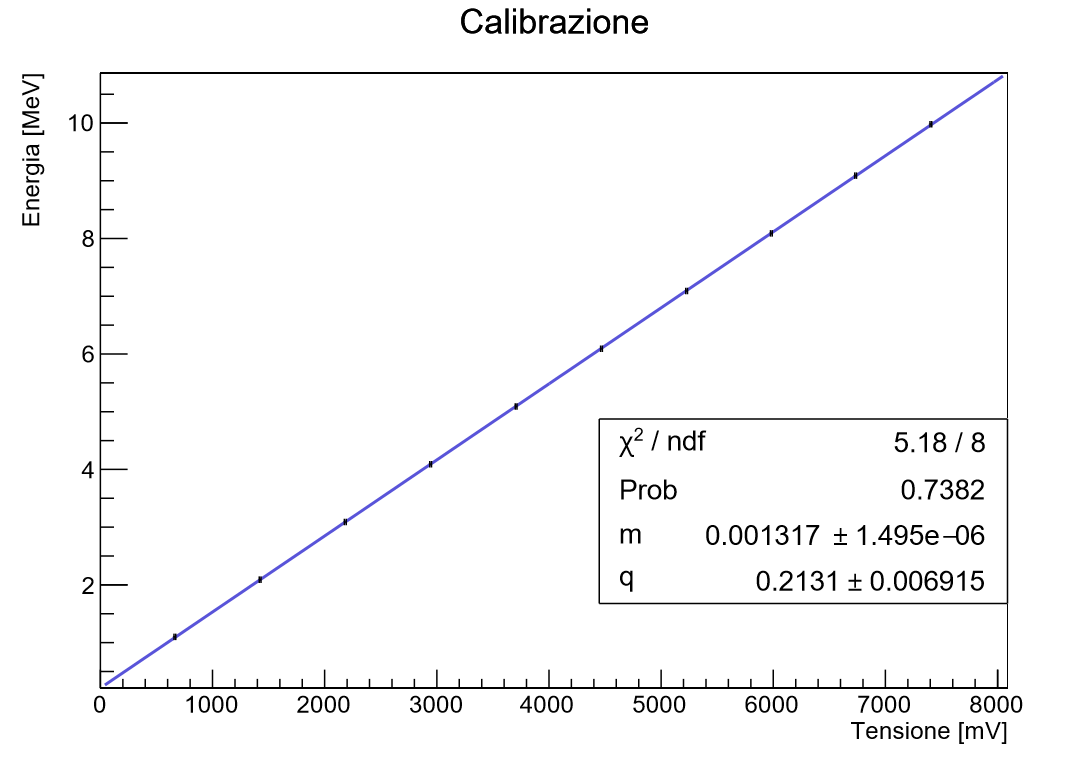
\includegraphics[scale=0.5]{rettacalibrazione.jpg}
\caption{Retta di calibrazione Energia vs. Picco}
\end{figure}

\subsection{Osservazioni}
Il grafico di calibrazione ottenuto mostra con chiarezza l'andamento lineare della relazione fra energia e tensione del picco. In particolar modo ci restituisce come risultato: 
\[
Energia = (1.32\cdot10^{-3})\cdot Picco \pm 10^{-6}
\]
\`E necessario però verificare l'attendibilit\`a dei risultati ottenuti andando a confrontare con lo spettro di una sorgente nota.
\section{Caratterizzazione con sorgente di 241-Am}
In questa parte successiva, nella camera viene inserita una sorgente di 241-Am, e ci\`o che in questo caso viene misurato \`e lo spettro in energia di questo materiale. Di seguito \`e riportato lo spettro, con una tabella che evidenzia i picchi relativi alle emissioni alfa della sorgente:\\

\begin{figure}[h!]
\centering
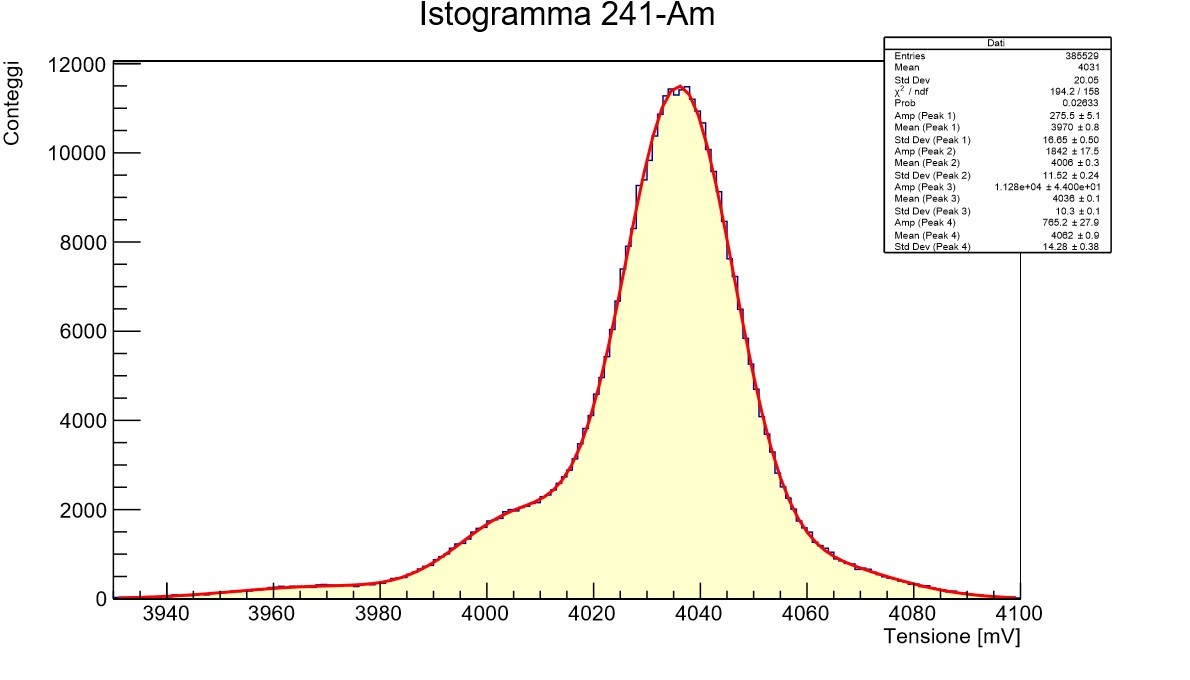
\includegraphics[scale=0.5]{istoame.jpg}
\caption{Spettro 241-Am}
\end{figure}

L'istogramma viene fittato con una somma di 4 gaussiane. Dal fit \`e possibile risalire ai 4 picchi di emissione del 241-Am. Utilizzando le energie di emissione tabulate, si costruisce una nuova curva di calibrazione:\\

\begin{figure}[H]
\centering
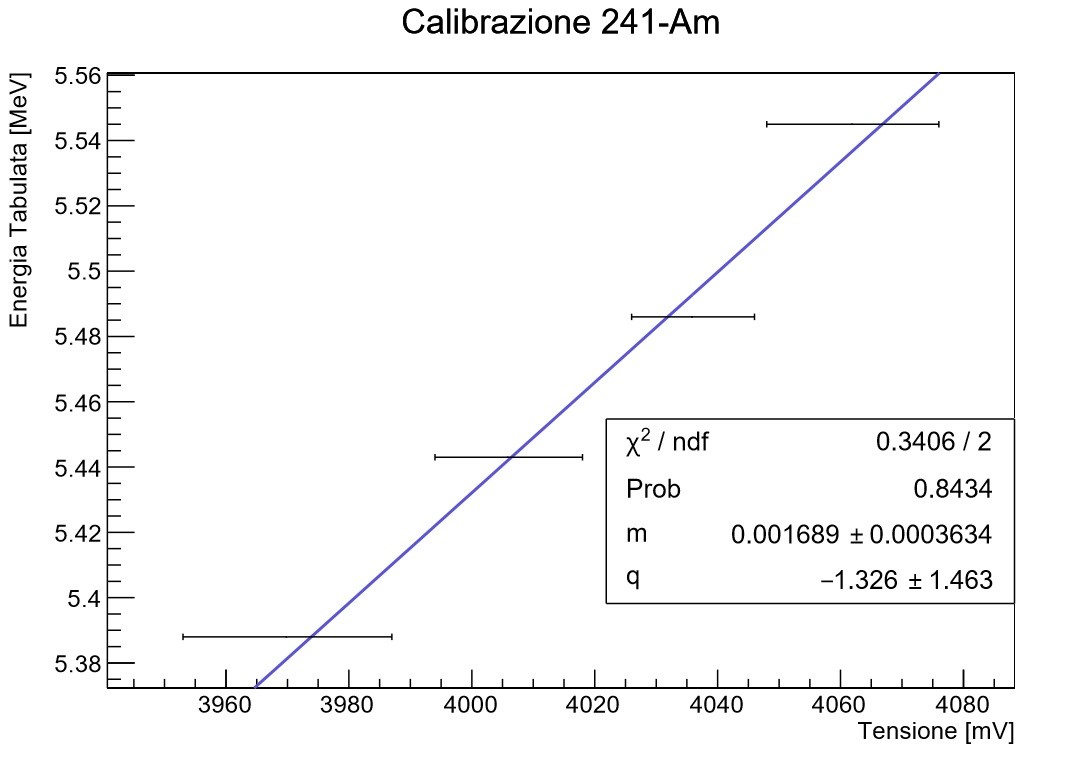
\includegraphics[scale=0.5]{rettaame.jpg}
\caption{Retta di calibrazione per il 241-Am}
\end{figure}

Di seguito invece, vengono riportate due tabelle: la prima mostra il confronto fra i parametri delle due rette di calibrazione, mentre la secondo il confronto fra i valori di energia tabulati dell'americio e quelli ottenuti attraverso la retta di calibrazione ottenuta nella prima parte:\\

\begin{center}
\begin{tabular}{ccccc}
\toprule
/ & Impulsatore & ErrImpulsatore & 241-Am & Err241-Am\\
\midrule
m & $1.32\cdot10^{-3}$ & $10^{-6}$ & $1.69\cdot10^{-3}$ & $3.63\cdot10^{-4}$\\
q & $2.13\cdot10^{-1}$ & $6.90\cdot10^{-3}$ & $1.32$ & $1.46$\\
\bottomrule
\end{tabular}\\
\end{center}
\begin{center}
\begin{tabular}{ccccc}
\toprule
Canale & E [KeV] & Errore [KeV] & Energia tabulata\\
\midrule
3970 & 5441.59 & 7.96 & 5388\\
4006 & 5489.00 & 7.98 & 5443\\
4036 & 5528.51 & 7.99 & 5486\\
4062 & 5562.75 & 8.01 & 5545\\
\bottomrule
\end{tabular}\\
\end{center}

Come ultima cosa, \`e possibile calcolare la risoluzione del rivelatore:\\

\begin{figure}[H]
\centering
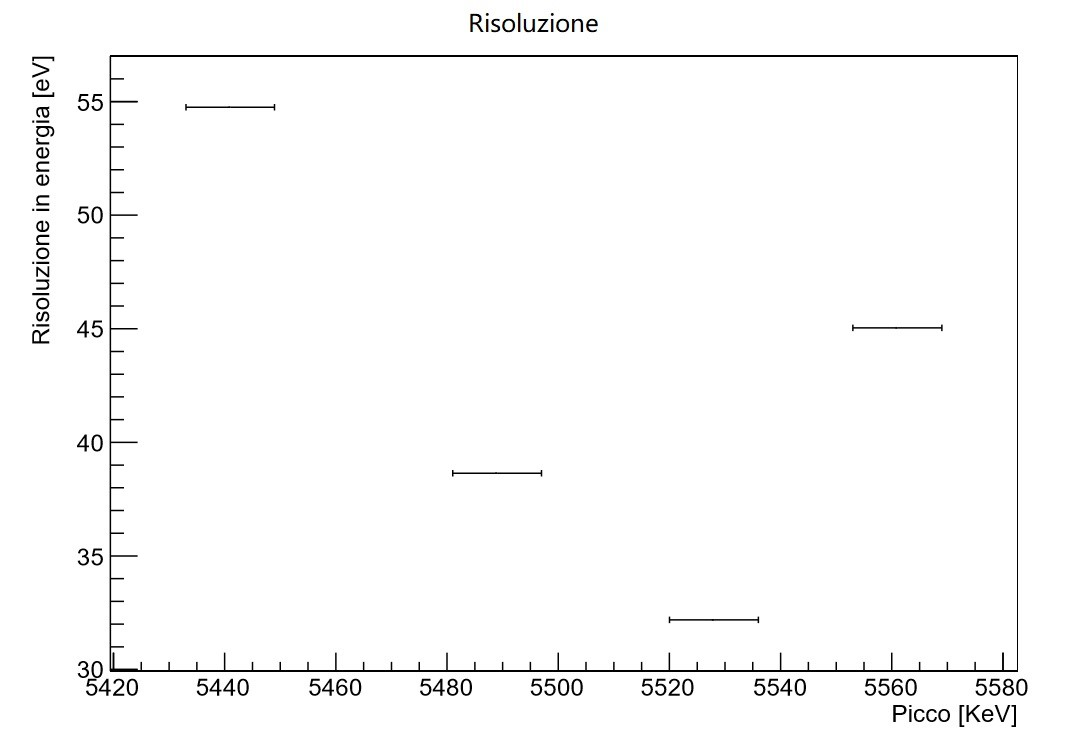
\includegraphics[scale=0.5]{risoluzione.jpg}
\caption{Risoluzione in funzione di E}
\end{figure}

\subsection{Osservazioni}
I dati che abbiamo elaborato mostrano alcune informazioni importanti. Innanzitutto le due rette di calibrazione, quella ottenuta nella prima parte attraverso l'impulsatore e quella ottenuta dallo studio dello spettro del 241-Am, non risultano compatibili: questo è evidenziato anche dalla incompatibilit\`a dei valori di energia tabulati corrispondenti ai picchi con quelli estrapolati dalla retta di calibrazione dell'impulsatore. Questo mostra come la calibrazione ottenuta con l'impulsatore, seppur importante per evidenziare la relazione lineare fra energia e tensione, non \`e molto precisa. La calibrazione con l'americio pu\`o essere in questo senso pi\`u attendibile. Questa incongruenza pu\`o essere legata a diversi fattori: innanzitutto il 241-Am ha solo 4 picchi, per altro molto vicini, e quindi difficilmente distinguibili. Infatti, come indicato, la risoluzione dell'apparato utilizzato è di circa 30/40 mV e ci\`o pu\`o influenzare la forma dello spettro. In pi\`u (...non so cosa altro mettere...)\\
Per quanto riguarda la risoluzione, essa \`e stata ottenuta dalla regola:
\[
R=\frac{FWHM}{E}=\frac{2.35\cdot\sigma}{E}
\]
L'andamento della risoluzione ottenuto \`e dunque consistente con quanto atteso per i primi 3 picchi: la risoluzione diminuisce all'aumentare dell'energia. Il fatto che il quarto ed ultimo punto non rispetti l'andamento pu\`o essere spiegato osservando lo spettro del 241-Am: l'ultimo picco, in corrispondeza del canale 4062, \`e quasi interamente coperto dal picco precendete, che corrisponde al decadimento dell'americio con il branching ratio più alto; questo rende difficile l'individuazione del picco stesso e della FWHM associata. 
\end{document} 